\notessection{Introduction to the Robot Operating System (ROS)}
This chapter introduces the fundamentals of the Robot Operating System (ROS)\cite{Joseph2018}\cite[\baselineskip]{QuigleyGerkeyEtAl2015}, a popular framework for creating robot software. Unlike what its name appears to suggest, ROS is not an operating system (OS). Rather, ROS is a ``middleware" that encompasses tools, libraries and conventions to operate robots in a simplified and consistent manner across a wide variety of robotic platforms. ROS is a critical tool in the field of robotics today, and is widely used in both academia and industry. 

This chapter begins by introducing specific challenges in robot programming that motivates the need for a middleware such as ROS.
Afterwards, a brief history of ROS will be presented to shed some light on its development and motivations for its important features.
Next, the fundamental operating structure of ROS will be discussed in further detail to provide insights into how ROS is operated on real robotic platforms. 
Lastly, specific features and tools of the ROS environment that greatly simplify robot software development will be presented.

\subsection{Challenges in Robot Programming}
Robot programming is a subset of computer programming, but it differs greatly from more classical software programming applications. One of the defining characteristics of robot programming is the need to manage many different individual hardware components that must operate in harmony (e.g. sensors and actuators on board the robot). In other words, robot software needs to not only run the ``brain" of the robot to make decisions, but also to handle multiple input and output devices at the same time. Therefore, the following features are needed for robot programming:

\begin{itemize}
    \item \textit{Multitasking:} Given a number of sensors and actuators on a robot, robot software needs to multitask and work with different input/output devices in different threads at the same time. Each thread needs to be able to communicate with other threads to exchange data. 
    
    \item \textit{Low level device control:} Robot software needs to be compatible with a wide variety of input and output devices: GPIO (general purpose input/output) pins, USB, SPI among others. C, C++ and Python all work well with low-level devices, so robot software needs to support either of these languages, if not all. 
    
    \item \textit{High level Object Oriented Programming (OOP):} In OOP, codes are encapsulated, inherited, and reused as multiple instances. Ability to reuse codes and develop programs in independent modules makes it easy to maintain code for complex robots.
    
    \item \textit{Availability of 3rd party libraries and community support:} Ample third-party libraries and community support not only expedite software development, but also facilitate efficient software implementation.
    
\end{itemize}

\subsection{Brief History of ROS}
Until the advent of ROS, it was impossible for various robotics developers to collaborate or share work among different teams, projects or platforms. In 2007, early versions of ROS started to be conceived with the Stanford AI Robot (STAIR) project, which had the following vision:

\begin{itemize}
    \item The new robot development environment should be free and open-source for everyone, and need to remain so to encourage collaboration of community members.
    \item The new platform should make core components of robotics -- from its hardware to library packages  -- readily available for anyone who intends to launch a robotics project.
    \item The new software development platform should integrate seamlessly with existing frameworks (OpenCV for computer vision, SLAM for localization and mapping, Gazebo for simulation, etc).
\end{itemize}

Development of ROS started to gain traction when Scott Hassan, a software architect and entrepreneur, and his startup  Willow Garage took over the project later that year to develop standardized robotics development platform. While mostly self-funded by Scott Hassan himself, ROS really satiated the dire needs for a standardized robot software development environment at the time. In 2009, ROS 0.4 was released, and a working ROS robot with a mobile manipulation platform called PR2 was developed. Eleven PR2 platforms were awarded to eleven universities across the country for further collaboration on ROS development, and in 2010 ROS 1.0 was released. Many of the original features from ROS 1.0 are still in use. In 2012, the Open Source Robotics Foundation (OSRF) started to supervise the future of ROS by supporting development, distribution, and adoption of open software and hardware for use in robotics research, education, and product development. In 2014 the first long-term support (LTS) release, ROS Indigo Igloo, became available.
Today, ROS has been around for 12 years, and the platform has become what is closest to the ``industry standard" in robotics. 

\subsubsection{Characteristics of ROS}
Building off of the initial needs first conceived by the STAIR project and the unique challenges persistent in robot programming, the ROS framework provides the following important capabilities:
\begin{figure*}[t] 
    \centering 
    \includegraphics[width=0.75\linewidth]{tex/figs/ch24_figs/ROS_modular.png}
    \caption{Modular software architecture designed to handle complexity of robot programming}
    \label{modularity} 
\end{figure*}

\begin{itemize}
    \item{\textit{Modularity:}} ROS handles complexity of a robot through modularity: Each robot component that performs separate functions can be developed independently in units called \textit{nodes} (Figure \ref{modularity}). Each node can share data with other nodes, and acts as the basic building blocks of ROS. Different functional capabilities on a robot can be developed in units called packages. Each package may contain a number of nodes that are defined from source code, configuration files, and data files. These packages can be distributed and installed on other computers. 

    \item{\textit{Message passing:}} ROS provides a message passing interface that allows nodes (i.e. programs) to communicate with each other. For example, one node might detect edges in a camera image, then send this information to an object recognition node, which in turn can send information about detected obstacles to a navigation module.
    
    \item{\textit{Built-in algorithms:}} A lot of popular robotics algorithms are already built-in and available as off-the-shelf packages: PID\footnote{\url{http://wiki.ros.org/pid}}, SLAM\footnote{\url{http://wiki.ros.org/gmapping}}, and path planners such as A* and Dijkstra\footnote[][2\baselineskip]{ \url{http://wiki.ros.org/global_planner}} are just a few examples. These built-in algorithms can significantly reduce time needed to prototype a robot.
  
    \item{\textit{Third-party libraries and community support:}} The ROS framework is developed with pre-existing third-party libraries in mind, and most popular libraries such as OpenCV for computer vision\footnote{\url{https://opencv.org}} and PCL\footnote{\url{http://pointclouds.org}} integrate simply with a couple lines of code. In addition, ROS is supported by active developers all over the world to answer questions (ROS Answers\footnote{\url{https://answers.ros.org/questions/}} or to discuss various topics and public ROS-related news\footnote{\url{https://discourse.ros.org}}. 
\end{itemize}

\subsection{Robot Programming with ROS}
Before jumping into using the functions and tools that ROS provides it is critical to understand a little more about how ROS operates. In particular, it is important to know that ROS uses a publish/subscribe (pub/sub) structure for communicating between different components or modules. This pub/sub structure (graphically shown in Figure \ref{chat_room}) allows messages to be passed in between components or modules through a shared virtual ``chat room''. To support this structure there are four primary components of ROS:
\begin{enumerate}
    \item Nodes: the universal name for the individual components or modules that need to send or receive information,
    \item Messages: the object for holding information that needs communicated between nodes,
    \item Topics: the virtual ``chat rooms'' where messages are shared,
    \item Master: the ``conductor'' that organizes the nodes and topics.
\end{enumerate}

\subsubsection{Nodes}

\begin{figure*}[t] 
    \centering 
    \includegraphics[width=0.65\linewidth]{tex/figs/ch24_figs/pub_sub.png}
    \caption{The ROS publish/subscribe (pub/sub) model.}
    \label{chat_room} 
\end{figure*}

\begin{definition}[Node]
A node\footnote{\url{http://wiki.ros.org/Nodes}} is a process that performs computation. Nodes are combined together to communicate with one another using streaming topics, RPC services, and the Parameter Server.
\end{definition}

Nodes are the basic building block of ROS that enables object-oriented robot software development. Each robot component is developed as an individual encapsulated unit of \textit{nodes}, which are later reused and inherited, and a typical robot control system will be comprised of many nodes. The use of independent nodes, and their ability to be reused and inherited, greatly simplifies the complexity of the overall software stack.

For example, suppose a robot is equipped with a camera and you want to find an object in the environment and drive to it. Examples of nodes that might be developed for this task are: a \texttt{camera} node that takes the image and pre-processes it, an \texttt{edge\_detection} node that takes the pre-processed image data and runs an edge detection algorithm, a \texttt{path\_planning} node that plans a path between two points, and so on.

At the individual level, nodes are responsible for \textbf{pub}lishing or \textbf{sub}scribing to certain pieces of information that are shared among all other nodes. In ROS, the pieces of information are called ``messages" and they are shared in virtual chat rooms called ``topics".

\subsubsection{Messages}

\begin{definition}[Messages]
Nodes communicate with each other by publishing simple data structures to topics. These data structures are called \textit{messages}\footnote{\url{http://wiki.ros.org/Messages}}.

\end{definition}
A message is defined by field types and field names. The field type defines the type of information the message stores and the name is how the nodes access the information. For example, suppose a node wants to publish two integers $x$ and $y$, a message definition might look like:
\begin{gencode}
int32 x
int32 y
\end{gencode}
where \texttt{int32} is the field type and \texttt{x/y} is the field name. While \texttt{int32} is a primitive field type, more complex field types can also be defined for specific applications. For example, suppose a sensor packet node publishes sensor data as an array of a user-defined \texttt{SensorData} object. This message, called \texttt{SensorPacket}, could have the following fields: 
\begin{gencode}
time            stamp
SensorData[]    sensors
uint32          length
\end{gencode}
In this case \texttt{SensorData} is a user-defined field type and the empty bracket \texttt{[]} is appended to indicate that field is an \textit{array} of \texttt{SensorType} objects.

More generally, field types can be either the standard primitive types (integer, floating point, boolean, etc.), arrays of primitive types, or other user-defined types. Messages can also include arbitrarily nested structures and arrays as well. Primitive message types available in ROS are listed below in Table \ref{table:Built-in Messages}. The first column contains the message type, the second column contains the serialization type of the data in the message and the third column contains the numeric type of the message in Python.

\begin{table}[ht]
\centering
\begin{tabular}{lll}
\hline
\textbf{Primitive Type} & \textbf{Serialization}          & \textbf{Python} \\ \hline
bool (1)                & unsigned 8-bit int              & bool            \\
int8                    & signed 8-bit int                & int             \\
uint8                   & unsigned 8-bit int              & int (3)         \\
int16                   & signed 16-bit int               & int             \\
uint16                  & unsigned 16-bit int             & int             \\
int32                   & signed 32-bit int               & int             \\
uint32                  & unsigned 32-bit int             & int             \\
int64                   & signed 64-bit int               & long            \\
uint64                  & unsigned 64-bit int             & long            \\
float32                 & 32-bit IEEE float               & float           \\
float64                 & 64-bit IEEE float               & float           \\
string                  & ascii string (4)                & str             \\
time                    & secs/nsecs unsigned 32-bit ints & rospy.Time      \\ \hline
\end{tabular}
\caption{Built-in ROS Messages} \label{table:Built-in Messages}
\end{table}

\subsubsection{Topics}
\begin{definition}[Topics]
Topics\footnote{http://wiki.ros.org/Topics} are named units over which nodes exchange messages.
\end{definition}

A given topic will have a specific message type associated with it, and any node that either publishes or subscribes to the topic must be equipped to handle that type of message. The command \texttt{rostopic type <topic>} can be used to see what kind of message is associated with a particular topic. Any number of nodes can publish or subscribe to a given topic.

Fundamentally, topics are for unidirectional, streaming communication. This is perhaps not well suited for all types of communication, such as communication that demands a response (i.e. a service routine). 

% As noted above, a publisher does not send messages until the topic is actually subscribed to. 
The \texttt{rostopic} command line tool can be used in several ways to monitor active topics/messages. Three of the most common rostopic commands are:
\begin{itemize}
    \item \texttt{rostopic list}: lists all active topics
    \item \texttt{rostopic echo < topic >}: prints messages received on topic
    \item \texttt{rostopic hz < topic >}: measures topic publishing rate
\end{itemize}
The last command is particularly useful in debugging responsiveness of an application.


\subsubsection{Master}

\begin{definition}[Master]
The master is a process that can run on any piece of hardware to track publishers and subscribers to topics as well as services in the ROS system.
\end{definition}

Master is responsible for assigning network addresses and enabling individual ROS nodes to locate one another, even if they are running on different computers. Once these nodes have located each other, the communication will be peer-to-peer, i.e., the master will not send nor receive the messages.
 
In any given ROS system, there is exactly one master running at any time. A unique feature of the master is that master does not need to exist within the robot's hardware as long as a network connection exists. The master can be facilitated remotely, on a much larger and more powerful computer.

\subsection{Writing a Simple Publisher Node and Subscriber Node}
\subsubsection{Publisher Node}
A simple publisher node that publishes String messages ten times per second can be implemented in Python via the following code\footnote{\url{http://wiki.ros.org/rospy_tutorials/Tutorials/WritingPublisherSubscriber}}:
\begin{python}
#!/usr/bin/env python
import rospy
from std_msgs.msg import String

def talker():
    rospy.init_node('talker', anonymous=True)
    pub = rospy.Publisher('chatter', String, queue_size=10)
    rate = rospy.get_param('~rate',1)
    ros_rate = rospy.Rate(rate)
    
    rospy.loginfo("Starting ROS node talker...")
    
    while not rospy.is_shutdown():
        msg= "Greetings humans!"
        
        pub.publish(msg)
        ros_rate.sleep()

if __name__ == '__main__':
    try:
        talker()
    except rospy.ROSInterruptException:
        pass

\end{python}
\vspace{\baselineskip}
\noindent
The first line:
\begin{pythonnoborder}
#!/usr/bin/env python
\end{pythonnoborder}
will be included in every Python ROS Node at the top of the file. This line makes sure your script is executed as a Python script. 

\vspace{\baselineskip}
\noindent
Next are the statements for importing specific Python libraries:
\begin{pythonnoborder}
import rospy
from std_msgs.msg import String
\end{pythonnoborder}
Note that the library \texttt{rospy} must be imported when writing a ROS Node. The \texttt{std\_msgs.msg} import enables the use of the \texttt{std\_msgs/String} message type (a simple string container) for publishing string messages.

\vspace{\baselineskip}
\noindent
Next is the definition of the ROS publisher node:
\begin{pythonnoborder}
rospy.init_node('talker', anonymous=True)
pub = rospy.Publisher('chatter', String, queue_size=10)
\end{pythonnoborder}
which creates a node called ``talker'' and defines the talker's interface to the rest of ROS. In particular:
\begin{itemize}
    \item \texttt{pub = rospy.Publisher("chatter", String, queue\_size=10)}  declares that the node is publishing to the ``chatter'' topic using the String message type. String here is actually the ROS datatype (\texttt{std\_msgs.msg.String}), and not Python's String datatype. The \texttt{queue\_size} argument limits the amount of queued messages that are allowed, for situations where a subscriber is not receiving the published messages fast enough.
    \item \texttt{rospy.init\_node(NAME, ...)} tells \texttt{rospy} the name of the node. Until \texttt{rospy} has this information, it cannot start communicating with the ROS Master. In this case, your node will take on the name talker. NOTE: the name must be a base name (i.e. it cannot contain any slashes ``/'').
    \item \texttt{anonymous=True} is a flag that tells \texttt{rospy} to generate a unique name for the node, since ROS requires that each node have a unique name. If a node with the same name comes up, it bumps the previous one so that malfunctioning nodes can easily be kicked off the network. This makes it easy to run multiple talker.py nodes.

    \item \texttt{anonymous = True} is another flag that ensures that the node has a unique name by adding random numbers to the end of NAME. 
\end{itemize} 
\noindent
The next lines of code:
\begin{pythonnoborder}
rate = rospy.get_param('~rate',1)
ros_rate = rospy.Rate(rate)
\end{pythonnoborder}
defines a ROS rate that can be used to time how often the node publishes. In particular, \texttt{rospy.get\_param(param\_name, default\_value)} reads a private ROS parameter (indicated by `\texttt{\mytilde}') called \texttt{rate}. This rate value is then used to create a \texttt{Rate} object \texttt{ros\_rate} in the second line.
The \texttt{Rate} object's \texttt{sleep()} method offers a convenient way for looping at the desired frequency. For example, if \texttt{rate} is 10, ROS should go through the loop 10 times per second (as long as the processing time does not exceed 1/10th of a second!).

\vspace{\baselineskip}
\noindent
The line:
\begin{pythonnoborder}
rospy.loginfo("Starting ROS node talker...")
\end{pythonnoborder}
performs three functions: it causes messages to get printed to screen, to be written to the Node's log file, and to be written to \texttt{rosout}. \texttt{rosout} is a handy tool for debugging that makes it possible to pull up messages using \texttt{rqt\_console} instead of having to find the console window with your Node's output.

\vspace{\baselineskip}
\noindent
The loop:
\begin{pythonnoborder}
while not rospy.is_shutdown():
    msg = "Greetings humans!"
    pub.publish(msg)
    ros_rate.sleep()
\end{pythonnoborder}
is a fairly standard rospy construct for first checking the \texttt{rospy.is\_shutdown()} flag and then doing work. The \texttt{is\_shutdown()} check is used to see if the program should exit (e.g. if there is a Ctrl-C interrupt). In this particular example, the ``work'' that is then performed inside of the loop is a call to \texttt{pub.publish(msg)}, which publishes a string to the ``chatter'' topic. The loop also calls \texttt{ros\_rate.sleep()} so that it sleeps just long enough to maintain the desired rate through the loop.

\subsubsection{Subscriber Node}
A subscriber node called \texttt{listener} can now be created to subscribe to the published ``chatter'' topic:
\begin{python}
!/usr/bin/env python
import rospy
from std_msgs.msg import String

def callback(msg):
    rospy.loginfo("Received: %s", msg.data)
    
def listener():
    rospy.init_node('listener', anonymous=True)
    rospy.Subscriber("chatter", String, callback)

    rospy.spin()

if __name__ == '__main__':
    listener()
\end{python}

The code for \texttt{listener.py} is similar to \texttt{talker.py}, except that a new callback-based mechanism for subscribing to messages is introduced.

\vspace{\baselineskip}
\noindent
First, the lines:
\begin{pythonnoborder}
    rospy.init_node('listener', anonymous=True)
    rospy.Subscriber("chatter", String, callback)
\end{pythonnoborder}
declare that the node subscribes to the ``chatter'' topic, which is of type \texttt{std\_msgs.msgs.String}. When new messages are received, the function \texttt{callback} is invoked with the message as the first argument.

\vspace{\baselineskip}
\noindent
The line:
\begin{pythonnoborder}
    rospy.spin()
\end{pythonnoborder}
then simply keeps the node from exiting until the node has been shutdown.

\subsubsection{Compiling and Running}
Once both the \texttt{talker.py} and \texttt{listener.py} nodes are ready, the \texttt{catkin} build system can be used to compile the code, and then both nodes can be run. Specifically, this is accomplished by running the following commands:
\begin{gencode}
$ cd ~/catkin_ws
$ catkin_make
$ python talker.py
$ python listener.py
\end{gencode}

\subsection{Other Features in ROS Development Environment }
\subsubsection{Launch files} 

As a robot project grows in scale, the number of nodes and configuration files grow very quickly. In practice, it could be very cumbersome to manually start up each individual node.
A \textit{launch file} provides a convenient way to start up multiple nodes and a master, as well as set up other configurations, all at the same time. 
\begin{definition}
Launch files are .launch files with a specific XML format that can be placed anywhere within a package directory to initialize multiple nodes, configuration files, and a master.
\end{definition}

While \texttt{.launch} files can be placed anywhere within a package directory, it is standard practice to create a \texttt{launch} folder inside the workspace directory to organize launch files.
Launch files must start and end with a pair of launch tags: \texttt{ <launch> ... </launch>}. To start a node using a launch file the following syntax should be used within the launch file:
\begin{gencode}
<node name="..." pkg="..." type="..."/>
\end{gencode}
In this line, \textbf{pkg} points to the package associated with the node that is to be launched, \textbf{type} refers to the name of the node executable file, and the name of the node can be overwritten with the \textbf{name} argument (this will take priority over the name that is given to the node in the code).
For example,
\begin{gencode}
<node name="bar1" pkg="foo_pkg" type="bar" />
\end{gencode}
launches the \texttt{bar} node from the \texttt{foo\_pkg} package with a new name, \texttt{bar1}. Alternatively,
\begin{gencode}
<node name="listener1" pkg="rospy_tutorials" type="listener.py"
     args="--test" respawn="true" />
\end{gencode}
launches the \texttt{listener1} node using the \texttt{listener.py} executable from the \texttt{rospy\_tutorials} package with the command-line argument \texttt{--test}. Additionally, if the node dies it will automatically be respawned.

There are other attributes that can be set when starting a node. While only \texttt{args} and \texttt{respawn} were introduced in this section, \url{http://wiki.ros.org/roslaunch/XML/node} is a great resource for additional parameters that can be used in the \texttt{<node>} tag.

\subsubsection{Catkin Workspace}

\texttt{catkin}\footnote{\texttt{catkin} refers to the tail-shaped flower cluster on willow trees -- a reference to Willow Garage where, \texttt{catkin} was created.} is a build system that compiles ROS packages. While \texttt{catkin}'s workflow\footnote{\url{http://wiki.ros.org/catkin/conceptual_overview}} is very similar to CMake's, \texttt{catkin} adds support for automatic `find package' infrastructure, for building multiple, dependent projects at the same time, and also supports both C and Python.

When developing with ROS, \texttt{catkin} should be run whenever a new project is started, or if there are any additions to packages. This is accomplished by creating a directory called \texttt{catkin\_ws} and then running the compile command \texttt{catkin\_make} in that directory:
\begin{gencode}
mkdir -p ~/catkin_ws/src  # builds the catkin_ws in the home dir
cd ~/catkin_ws            # change current directory to catkin_ws
catkin_make               # run catkin
\end{gencode}

\begin{figure*}[t] 
    \centering 
    \includegraphics[width=0.75\linewidth]{tex/figs/ch24_figs/catkin_ws.png}
    \caption{Components of an example ROS package named \texttt{mypackage} in a \texttt{catkin} workspace.}
    \label{catkin} 
\end{figure*} 

Once the \texttt{catkin} workspace is compiled, it will automatically contain the files \texttt{CMakeLists.txt} and \texttt{package.xml}. There are other sub-folders in \texttt{catkin\_ws} as well, as shown in Figure \ref{catkin}, which can be changed as needed.

\subsubsection{Debugging}
Robot programming requires a lot of debugging. There are a few ways to debug your robot software, including (but not limited to): 
\begin{itemize}
    \item \verb|rostopic|: a tool that monitors ROS topics in the command line,
    \item \verb|rospy.loginfo()|: starts a background process that writes ROS messages to a ROS logger, viewable through a program such as \verb|rqt_console|,
    \item \verb|rosbag|: provides a convenient way to record a number of ROS topics for playback,
    \item \texttt{pdb}: provides a useful tool for debugging python scripts.
\end{itemize}

\subsubsection{Gazebo} 
Gazebo\footnote{\url{http://gazebosim.org}} is a popular 3D dynamic simulator with the ability to accurately and efficiently simulate robots in complex environments (see Figure \ref{gazebo_screenshot}). While similar to game engines, Gazebo offers a higher fidelity physics simulation, a suite of sensors models, and interfaces for both users and programs. Gazebo can be used in any stage of robot development, from testing algorithms to running regression testing in realistic scenarios.
Integration of Gazebo with ROS is possible via \texttt{gazebo\_ros\_pkgs} package. 
 
\begin{figure}[ht] 
    \centering 
    \includegraphics[width=0.9\linewidth]{tex/figs/ch24_figs/Gazebo.PNG}
    \caption{Screenshot of a scene in Gazebo.}
    \label{gazebo_screenshot} 
\end{figure} 
